% article: fontspec, TikZ and pgfplots, graphicx, float
\documentclass{article}
\usepackage{fontspec}
\setmainfont{texgyreschola}[Extension=.otf, UprightFont=*-regular, BoldFont=*-bold, ItalicFont=*-italic, BoldItalicFont=*-bolditalic]
\usepackage{graphicx}
\usepackage{tikz}
\usepackage{pgfplots}
\pgfplotsset{compat=1.18}
\begin{document}
\section{Figures}
Figure~\ref{f:plot} shows a pgfplots plot and Figure~\ref{f:img} an image.
\begin{figure}[h]\centering
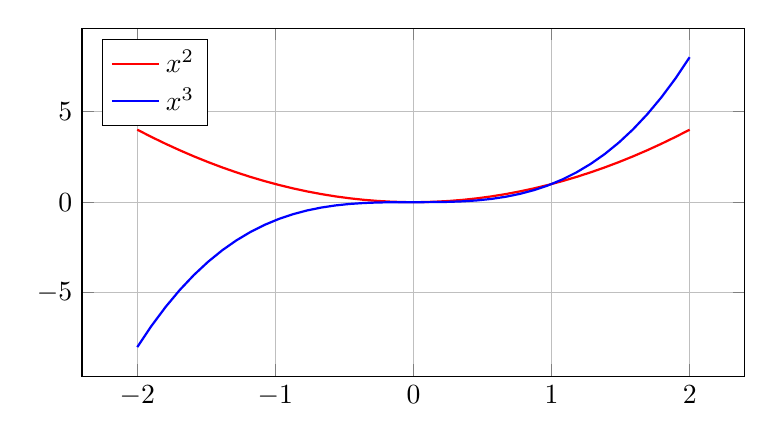
\begin{tikzpicture}
\begin{axis}[width=10cm,height=6cm,legend pos=north west,grid=major]
\addplot[red,thick,domain=-2:2,samples=40]{x^2};
\addplot[blue,thick,domain=-2:2,samples=40]{x^3};
\legend{$x^2$,$x^3$}
\end{axis}
\end{tikzpicture}
\caption{Two curves.}\label{f:plot}
\end{figure}
\begin{figure}[h]\centering
\includegraphics[width=.4\linewidth]{example-image-b}\hspace{1em}
\begin{tikzpicture}\draw[fill=orange!30] (0,0) circle (1); \node at (0,0) {Ω};\end{tikzpicture}
\caption{An image and a TikZ picture with a Unicode label.}\label{f:img}
\end{figure}
\end{document}
